\date{}
\title{}
\date{}
\begin{document}
\begin{frame}
    \titlepage
\end{frame}

\input{../common/listingsLib}
\newcommand{\z}[2]{\only<#1->{\myemph<#1>{#2}}}
\newcommand{\zz}[3]{\only<#1-#2>{\myemph<#1>{#3}}}
\newcommand{\zzx}[3]{\only<#1-#2>{#3}}
\newlength{\oneZero}
\settowidth{\oneZero}{\small\tt 0}
\newlength{\twoZeroes}
\settowidth{\twoZeroes}{\small\tt 00}

\usetikzlibrary{calc}

\begin{frame}{last time}
    \begin{itemize}
    \item simulated direct-mapped caches
    \item conflict misses happening `accidentally'
    \item adding associativity
        \begin{itemize}
        \item multiple blocks per set
        \item mutliple tags to check
        \end{itemize}
    \item replacement policies / least recently used
        \begin{itemize}
        \item LRU tracking via updates on each access
        \end{itemize}
    \item understanding how C code accesses data caches
    \end{itemize}
\end{frame}

\subsection{array misses warmup}
\input{../caching/arrayMissesWarmupEx}

\subsection{array misses warmup (2 set)}
\begin{frame}[fragile,label=arrayMissesWarmup3]{C and cache misses (warmup 3)}
\begin{lstlisting}[style=size10]
int array[8];
...
int even_sum = 0, odd_sum = 0;
even_sum += array[0];
odd_sum += array[1];
even_sum += array[2];
odd_sum += array[3];
even_sum += array[4];
odd_sum += array[5];
even_sum += array[6];
odd_sum += array[7];
\end{lstlisting}
\begin{itemize}
\item {\small
Assume everything but {\tt array} is kept in registers (and the compiler does not do
anything funny), and array[0] at beginning of cache block.}
\item How many data cache misses on a \textbf{2}-set direct-mapped cache with 8B blocks?
\end{itemize}
\end{frame}

\begin{frame}<0>[fragile,label=arrayMissesWarmup3Answers]{exercise solution}
\newcommand{\mywidth}{0.39}
\begin{tikzpicture}
    \foreach \offset in {-2,-1,0,1,2,...,31,32,33} {
        \draw[black!25,thin] (\offset * \mywidth, 0) rectangle ++(\mywidth, -1);
    }
    \node[font=\large,anchor=east] at (-2 * \mywidth, -.5) {\ldots};
    \node[font=\large,anchor=west] at (34 * \mywidth, -.5) {\ldots};
    \begin{scope}
    \clip (-2.1 * \mywidth, .2) rectangle (34.1 * \mywidth, -1.1);
    \foreach \offset/\name in {8/0,12/1,16/2,20/3,24/4,28/5,32/6} {
        \draw[thin,fill=blue!10] (\offset * \mywidth, 0) rectangle ++(\mywidth * 4, -1)
            node[fill=none,opacity=1.0,black,midway,font=\fontsize{9}{10}\tt\selectfont] {array[\name]};
    }
    \foreach \offset in {-8,0,8,16,24,32} {
        \draw[ultra thick,red!30!black] (\offset * \mywidth, 0)
            rectangle ++(\mywidth * 8, -1);
    }
    \end{scope}
        \draw[very thick, decorate, decoration={brace}] (8 * \mywidth, 0.05) -- ++(8 * \mywidth, 0)
            node[inner sep=0mm,above=1mm,midway,align=center,font=\small] {one cache block \\
                                (index 0)};
        \begin{visibleenv}<2->
        \draw[very thick, decorate, decoration={brace}] (16 * \mywidth, 0.05) -- ++(8 * \mywidth, 0)
            node[inner sep=0mm,above=1mm,midway,align=center,font=\small] {one cache block \\
                                (index 1)};
        \draw[very thick, decorate, decoration={brace}] (24 * \mywidth, 0.05) -- ++(8 * \mywidth, 0)
            node[inner sep=0mm,above=1mm,midway,align=center,font=\small] {one cache block \\
                                (index 0)};
        \draw[very thick, decorate, decoration={brace}] (0 * \mywidth, 0.05) -- ++(8 * \mywidth, 0)
            node[inner sep=0mm,above=1mm,midway,align=center,font=\small] {one cache block \\
                                (index 1)};
        \end{visibleenv}
    \begin{visibleenv}<3->
    \tikzset{
        set both/.style={alt=<5-7>{nodes={fill=red!10}}},
        set 0/.style={
            alt=<5-6>{nodes={fill=red!10}},
            alt=<7>{opacity=0.1},
        },
        set 1/.style={
            alt=<5-6>{opacity=0.1},
            alt=<7>{nodes={fill=red!10}},
        },
    }
    \matrix[tight matrix,
        nodes={minimum height=0.5cm,font=\fontsize{8}{9}\selectfont},
        column 1/.append style={nodes={text width=4cm}},
        column 2/.append style={nodes={text width=5cm,font=\fontsize{10}{11}\tt\selectfont,set 0}},
        column 3/.append style={nodes={text width=5cm,font=\fontsize{10}{11}\tt\selectfont,set 1}},
        row 1/.append style={nodes={font=\fontsize{9}{10}\bfseries\selectfont}},
        row 2/.append style={set both},
        row 3/.append style={set 0},
        row 4/.append style={set 0},
        row 5/.append style={set 1},
        row 6/.append style={set 1},
        row 7/.append style={set 0},
        row 8/.append style={set 0},
        row 9/.append style={set 1},
        row 10/.append style={set 1},
        anchor=north west] at (-1, -1) {
        memory access \& set 0 afterwards \& set 1 afterwards \\ 
        --- \& (empty) \& (empty) \\
        read \lstinline|array[0]| (miss) \& \{array[0], array[1]\} \& (empty) \\
        read \lstinline|array[1]| (hit) \& \{array[0], array[1]\} \& (empty) \\
        read \lstinline|array[2]| (miss) \& \{array[0], array[1]\} \& \{array[2], array[3]\} \\
        read \lstinline|array[3]| (hit) \& \{array[0], array[1]\} \& \{array[2], array[3]\} \\
        read \lstinline|array[4]| (miss) \& \{array[4], array[5]\} \& \{array[2], array[3]\} \\
        read \lstinline|array[5]| (hit) \& \{array[4], array[5]\} \& \{array[2], array[3]\} \\
        read \lstinline|array[6]| (miss) \& \{array[4], array[5]\} \& \{array[6], array[7]\} \\
        read \lstinline|array[7]| (hit) \& \{array[4], array[5]\} \& \{array[6], array[7]\} \\
    };
    \end{visibleenv}
    \begin{visibleenv}<4-5>
        \node[align=left,draw=red,ultra thick,fill=white] at (6.5, -0.25) {
            observation: what happens in set 0 doesn't affect set 1 \\
            \myemph<5>{when evaluating set 0 accesses,} \\
            \myemph<5>{can ignore non-set 0 accesses/content}
        };
    \end{visibleenv}
\end{tikzpicture}
\end{frame}

\iftoggle{heldback}{}{
\againframe<1-3>{arrayMissesWarmup3Answers}
\againframe<4->{arrayMissesWarmup3Answers}
}


\input{../caching/arrayMissesWarmup2SetEx2}

\subsection{array misses and cache results}
\begin{frame}[fragile,label=arrayMissesWarmup5]{C and cache misses (warmup 5)}
\begin{lstlisting}[style=smaller]
int array[1024]; /* assume aligned */
int even_sum = 0, odd_sum = 0;
even_sum += array[0];
even_sum += array[2];
even_sum += array[512];
even_sum += array[514];
odd_sum += array[1];
odd_sum += array[3];
odd_sum += array[511];
odd_sum += array[513];
\end{lstlisting}
\begin{itemize}
\item {\small
Assume everything but {\tt array} is kept in registers (and the compiler does not do
anything funny).}
\item observation: array[0] and array[512] exactly 2KB apart
\item How many data cache misses on a 2KB direct mapped cache with 16B blocks
\end{itemize}
\end{frame}

\begin{frame}[fragile,label=arrayMissesWarmup6]{C and cache misses (warmup 6)}
\begin{lstlisting}[style=smaller]
int array[1024]; /* assume aligned */
int even_sum = 0, odd_sum = 0;
even_sum += array[0];
even_sum += array[2];
even_sum += array[500];
even_sum += array[502];
odd_sum += array[1];
odd_sum += array[3];
odd_sum += array[501];
odd_sum += array[503];
\end{lstlisting}
\begin{itemize}
\item {\small
Assume everything but {\tt array} is kept in registers (and the compiler does not do
anything funny).}
\item observation: array[0] and array[500] exactly 2KB apart
\item How many data cache misses on a 2KB direct mapped cache with 16B blocks
\end{itemize}
\end{frame}


\subsection{array misses and skipping around}
\begin{frame}<1>[fragile,label=arrayMissesSkip]{misses with skipping}
\begin{lstlisting}
int array1[512]; int array2[512];
...
for (int i = 0; i < 512; i += 1)
    sum += array1[i] * array2[i];
}
\end{lstlisting}
    \begin{itemize}
        \item {\small
    Assume everything but {\tt array1}, {\tt array2} is kept in registers (and the compiler does not do
    anything funny).
        }
    \item
About how many \textit{data cache misses} on a 2KB direct-mapped cache with 16B cache blocks? \\
Hint: depends on relative placement of array1, array2
\end{itemize}
\end{frame}

\begin{frame}{best/worst case}
\begin{itemize}
\item \texttt{array1[i]} and \texttt{array2[i]} always different sets:
    \begin{itemize}
    \item 2 misses every 4 \texttt{i}
    \item = distance from array1 to array2 not multiple of \# sets $\times$ bytes/set
    \end{itemize}
\item \texttt{array1[i]} and \texttt{array2[i]} same sets:
    \begin{itemize}
    \item 2 misses every \texttt{i}
    \item = distance from array1 to array2 is multiple of \# sets $\times$ bytes/set
    \end{itemize}
\end{itemize}
\end{frame}

\begin{frame}{worst case in practice?}
    \begin{itemize}
    \item two rows of matrix?
    \item often sizeof(row) bytes apart
    \item if the row size is multiple of number of sets $\times$ bytes per block, oops!
    \end{itemize}
\end{frame}


\subsection{mapping misses to sets (3-way)}
\input{../caching/setMappingDiag3}

\section{revisiting array misses and skips}
\againframe<2>{arrayMissesSkip}

\section{array misses and associative caches?}
\begin{frame}[fragile,label=arrayMissesAssocBig1]{C and cache misses (assoc)}
\begin{lstlisting}[style=smaller]
int array[1024]; /* assume aligned */
int even_sum = 0, odd_sum = 0;
even_sum += array[0];
even_sum += array[2];
even_sum += array[512];
even_sum += array[514];
odd_sum += array[1];
odd_sum += array[3];
odd_sum += array[511];
odd_sum += array[513];
\end{lstlisting}
{\small
Assume everything but {\tt array} is kept in registers (and the compiler does not do
anything funny).\\
opbservation: array[0], array[256], array[512], array[768] in same set}
\begin{itemize}
\item How many data cache misses on a 2KB 2-way set associative cache with 16B blocks
\end{itemize}
\end{frame}

\begin{frame}[fragile,label=arrayMissesAssocBig2]{C and cache misses (assoc)}
\begin{lstlisting}[style=smaller]
int array[1024]; /* assume aligned */
int even_sum = 0, odd_sum = 0;
even_sum += array[0];
even_sum += array[256];
even_sum += array[512];
even_sum += array[768];
odd_sum += array[1];
odd_sum += array[257];
odd_sum += array[513];
odd_sum += array[769];
\end{lstlisting}
{\small
Assume everything but {\tt array} is kept in registers (and the compiler does not do
anything funny).\\
observation: array[0], array[256], array[512], array[768] in same set}
\begin{itemize}
\item How many data cache misses on a 2KB 2-way set associative cache with 16B blocks?
\end{itemize}
\end{frame}


\section{simulated misses with set-assoc. caches}
\begin{frame}{simulated misses: BST lookups}
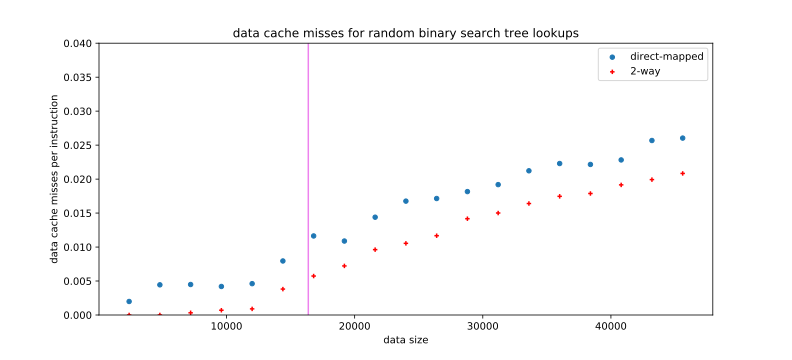
\includegraphics[width=\textwidth]{../caching/bst-both}
\end{frame}

\begin{frame}{simulated misses: matrix multiplies}
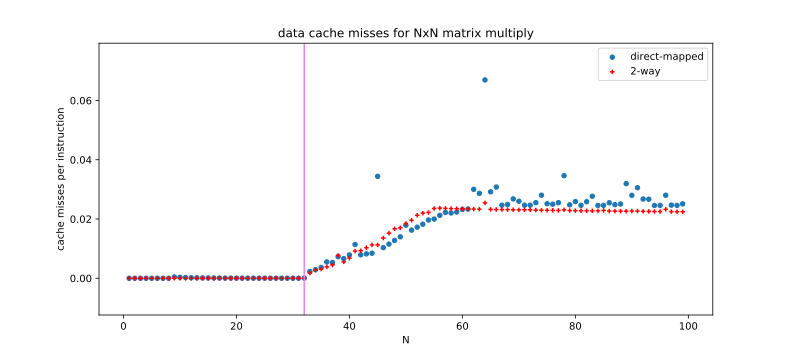
\includegraphics[width=\textwidth]{../caching/mm-both}
\end{frame}


\section{options for handling cache writes}
\input{../caching/writePolicy}

\subsection{exercise: write/replacement policies}
\input{../caching/writeReplaceExercise}

\subsection{fast writes: write buffers}
\input{../caching/fastWrites}

\subsection{briefly, cache tradeoffs}
\begin{frame}{cache tradeoffs briefly}
    \begin{itemize}
    \item deciding cache size, associativity, etc.?
    \item lots of tradeoffs:
        \begin{itemize}
        \item more cache hits v. slower cache hits?
        \item faster cache hits v. fewer cache hits?
        \item (N+1)th-level cache v. larger Nth level cache?
        \item \ldots
        \end{itemize}
    \item details depend on programs run
        \begin{itemize}
        \item how often is same block used again?
        \item how often is same index bits used?
        \item how much \{temporal,spatial\} locality to take advantage of?
        \end{itemize}
    \item simulation to assess impact of designs
    \end{itemize}
\end{frame}


\section{TLB}
\input{../vm/twoLevelPtLib}
\subsection{review: page table lookup (1)}
\input{../vm/twoLevelPTAlt}

\subsection{review: page table lookup (2)}
\againframe<7>{twoLevelPtLookup}

\subsection{why cache page table entries?}
\input{../caching/tlbWhy}

\subsection{how TLB fits in page table lookup}
\input{../caching/tlbMulti}

\subsection{how TLBs are organized}

\usetikzlibrary{decorations,decorations.pathreplacing,circuits.logic.US,matrix,positioning}
\usetikzlibrary{circuits.logic.mux}
\begin{frame}[fragile,label=tlbOrg]{TLB organization (2-way set associative)}
\vspace{1cm}
\begin{tikzpicture}[circuit logic US]
\tikzset{
    myline/.style={-latex,thick},
    myline thin/.style={-latex,thin},
    myline bus/.style={-latex,ultra thick},
    myline no arrow/.style={thick},
    offsetColor/.style={color=yellow!30!black},
    tagColor/.style={color=green!60!black},
    tagStoreFill/.style={fill=green!20},
    tagColorFill/.style={tagColor,fill=green!60!black},
    dataColor/.style={color=blue!60!black},
    dataColorFill/.style={tagColor,fill=blue!60!black},
    dataStoreFill/.style={fill=blue!20},
    triangle down/.style = {draw,regular polygon, regular polygon sides=3, shape border rotate=180},
    N/.style={draw=none,fill=none},
}
\matrix[tight matrix,
        nodes={draw,
               font=\small\tt,
               text depth=0.2ex,
               text height=1.4ex,
        },
        row 1/.style={nodes={font=\small\bfseries,minimum height=1cm,text depth=0.6cm}},
        column 1/.style={nodes={text width=1cm,align=center}},
        column 2/.style={nodes={text width=1cm,tagColor,tagStoreFill}},
        column 3/.style={nodes={text width=1.65cm,dataColor,dataStoreFill}},
        column 4/.style={nodes={text width=1cm,dataColor,dataStoreFill}},
        column 5/.style={nodes={text width=1cm,dataColor,dataStoreFill}},
        column 6/.style={nodes={text width=.1cm,draw=none}},
        column 7/.style={nodes={text width=1cm,align=center}},
        column 8/.style={nodes={text width=1cm,tagColor,tagStoreFill}},
        column 9/.style={nodes={text width=1.65cm,dataColor,dataStoreFill}},
        column 10/.style={nodes={text width=1cm,dataColor,dataStoreFill}},
        column 11/.style={nodes={text width=1cm,dataColor,dataStoreFill}},
        ] (cache) {
    valid \& tag \&  physical page \# \& write \& \ldots \& ~ \& valid \& tag \& physical page \# \& write  \& \ldots \\
    |[N]| \ldots \& |[N]| \ldots \& |[N]| \ldots \& |[N]| \ldots \& |[N]| \ldots \& ~ \&
    |[N]| \ldots \& |[N]| \ldots \& |[N]| \ldots \& |[N]| \ldots \& |[N]| \ldots \\
    1  \& 10 \& 0x123 \& 1 \& ~ \& ~ \& 1 \& 11 \& 0x12F \& 1 \& ~ \\
    ~ \&  ~    \& ~     \& ~ \&  ~ \& ~\& ~ \& ~ \& ~    \& ~     \& ~  \\
    |[alias=bottom-validA]| ~ \&  |[alias=bottom-tagA]| ~ \& |[alias=bottom-ppnA]| ~ \& |[alias=bottom-writeA]| ~  \& |[alias=bottom-miscA]| ~ \& ~ \&
    |[alias=bottom-validB]| ~ \& |[alias=bottom-tagB]| ~ \& |[alias=bottom-ppnB]| ~  \& |[alias=bottom-writeB]| ~  \& 
        |[alias=bottom-miscB]| ~\\
};
\begin{scope}[every node/.style={draw,rectangle,dashed,inner xsep=0pt,outer sep=0pt,font=\tt}]
\node (idx) at ([yshift=.75cm,xshift=-.6cm]cache.north west){100};
\node[left=0cm of idx,tagColor] (tag) {11};
\end{scope}
\node[right=0cm of idx,offsetColor,inner xsep=0pt,outer sep=0pt,font=\tt] (po) {010110};
\draw[thick,dashed,-latex] (idx) |- ([xshift=-.25cm]cache-3-1.west) node[near start,font=\small,fill=white,inner sep=2pt,xshift=-.3cm] {index};
\draw[very thick,decorate,decoration={brace,mirror},overlay] ([xshift=-.1cm]cache-2-1.north west) -- ([xshift=-.1cm]cache-5-1.south west);

\draw[thick,dashed,-latex,tagColor] (tag) |- ([yshift=-1cm]cache-5-2.south) coordinate (tag cmp 1);
\draw[thick,dashed,-latex,tagColor] (cache-5-2.south) -- (tag cmp 1);
\draw[thick,dashed,-latex,tagColor] (tag) |- ([yshift=-2cm]cache-5-8.south) coordinate (tag cmp 2)
    node[midway,fill=white] {tag};
\draw[thick,dashed,-latex,tagColor] (cache-5-8.south) -- (tag cmp 2);

\node[right=.25cm of po,inner xsep=0pt,outer sep=0pt] {(program address)};

\draw[very thick,decorate,decoration={brace},overlay] ([yshift=.05cm]tag.north west) -- ([yshift=.05cm]idx.north east)
    node [midway,above,alt=<2>{red},overlay] {VPN};

\draw[very thick,black!80,decorate,decoration={brace},overlay] ([yshift=.05cm]po.north west) -- ([yshift=.05cm]po.north east)
    node [midway,above,font=\small,alt=<3>{red},overlay] {page offset};


\begin{visibleenv}<4>
\node[fit=(cache-3-3) (cache-3-5),inner sep=1pt,red,draw,line width=1pt,label={[fill=white,fill opacity=0.9]north:page table entry}] {};
\end{visibleenv}

\begin{visibleenv}<5>
\node[fit=(cache-3-1) (cache-3-11),inner sep=1pt,red,draw,line width=3pt] {};
\end{visibleenv}
\end{tikzpicture}
\end{frame}
 % FIXME: emphasize that AFTER this is normal cache access

\subsection{exercise: TLB access pattern}
\input{../caching/tlbAccessExPrep}
\input{../caching/tlbAccessEx}


\section{backup slides}
\begin{frame}{backup slides}
\end{frame}


\section{backup slides --- general}

\begin{frame}[fragile,label=arrayMissesOddEven1]{arrays and cache misses (1)}
\begin{lstlisting}
int array[1024]; // 4KB array
int even_sum = 0, odd_sum = 0;
for (int i = 0; i < 1024; i += 2) {
    even_sum += array[i + 0];
    odd_sum +=  array[i + 1];
}
\end{lstlisting}
    \begin{itemize}
        \item {\small
Assume everything but {\tt array} is kept in registers (and the compiler does not do
            anything funny).}
\item
How many \textit{data cache misses} on initially empty 2KB direct-mapped cache with 16B cache blocks?
    \end{itemize}
\end{frame}

\begin{frame}<1>[fragile,label=arrayMissesOddEven2]{arrays and cache misses (2)}
\begin{lstlisting}
int array[1024]; // 4KB array
int even_sum = 0, odd_sum = 0;
for (int i = 0; i < 1024; i += 2)
    even_sum += array[i + 0];
for (int i = 0; i < 1024; i += 2)
    odd_sum +=  array[i + 1];
\end{lstlisting}
    \begin{itemize}
        \item {\small
    Assume everything but {\tt array} is kept in registers (and the compiler does not do
    anything funny).
        }
    \item
How many \textit{data cache misses} on initially empty 2KB direct-mapped cache with 16B cache blocks?
            \only<2->{Would a set-associtiave cache be better?}
    \end{itemize}
\end{frame}

\begin{frame}[fragile,label=arrayMissesOddEven3]{arrays and cache misses (2b)}
\begin{lstlisting}
int array[1024]; // 4KB array
int even_sum = 0, odd_sum = 0;
for (int i = 0; i < 1024; i += 2)
    even_sum += array[i + 0];
for (int i = 0; i < 1024; i += 2)
    odd_sum +=  array[i + 1];
\end{lstlisting}
    \begin{itemize}
        \item {\small
    Assume everything but {\tt array} is kept in registers (and the compiler does not do
    anything funny).
        }
    \item
        How many \textit{data cache misses} on initially empty \myemph{4KB} direct-mapped cache with 16B cache blocks?
    \end{itemize}
\end{frame}

\begin{frame}[fragile,label=arrayMisses4]{arrays and cache misses (3)}
\begin{lstlisting}
int array[1024]; // 4KB array
int sum;
for (int i = 8; i < 1016; i += 1) {
    int local_sum = 0;
    for (int j = i - 8; j < i + 8; j += 1) {
        local_sum += array[i] * (j - i);
    }
    sum += (local_sum - array[i]);
}
\end{lstlisting}
    \begin{itemize}
        \item {\small
    Assume everything but {\tt array} is kept in registers (and the compiler does not do
    anything funny).
        }
    \item
        How many \textit{data cache misses} on initially empty \myemph{2KB} direct-mapped cache with 16B cache blocks?
    \end{itemize}
\end{frame}



\subsection{inclusive v exclusive}
\usetikzlibrary{patterns}
\begin{frame}{inclusive versus exclusive}
\begin{tikzpicture}
\tikzset{
    >=Latex,
    connect/.style={<->,ultra thick},
    cache/.style={draw,very thick},
    fill 1/.style={pattern color=blue!50!black,pattern=crosshatch},
    fill 2/.style={pattern color=orange,pattern=dots},
}
\node (l2 incl label) at (2.5, 6.5) {L2 inclusive of L1};
\node[font=\small,anchor=north,align=center] at (l2 incl label.south) {
    everything in L1 cache duplicated in L2 \\
    adding to L1 also adds to L2
};
\node[anchor=south]  at (1, 2) {L1 cache};
\node[anchor=south]  at (4, 4) {L2 cache};
\draw[cache] (0, 0) rectangle ++(2, 2);
\path[fill 1] (0, 0) rectangle ++(2, 2);
\path[fill 2] (3, -1.5) rectangle ++(2,1);
\path[fill 1] (3, -0.5) rectangle ++(2, .5);
\path[fill 2] (3, 0) rectangle ++(2,.25);
\path[fill 1] (3, 0.25) rectangle ++(2, .3);
\path[fill 2] (3, 0.55) rectangle ++(2,.65);
\path[fill 1] (3, 1.2) rectangle ++(2, .6);
\path[fill 2] (3, 1.8) rectangle ++(2,.2);
\path[fill 1] (3, 2) rectangle ++(2, .6);
\path[fill 2] (3, 2.6) rectangle ++(2,1.4);
\draw[cache] (3, -1.5) rectangle ++(2, 5.5);

\begin{scope}[xshift=8cm]
\node (l2 excl label) at (2.5, 6.5) {L2 exclusive of L1};
\node[font=\small,anchor=north,align=center] at (l2 excl label.south) {
    L2 contains different data than L1 \\
    adding to L1 must remove from L2 \\
    probably evicting from L1 adds to L2
};
\node[anchor=south]  at (1, 2) {L1 cache};
\node[anchor=south]  at (4, 4) {L2 cache};
\path[fill 1] (0, 0) rectangle ++(2, 2);
\draw[cache] (0, 0) rectangle ++(2, 2);
\draw[cache,fill 2] (3, -1.5) rectangle ++(2, 5.5);
\end{scope}
\begin{visibleenv}<2>
    \draw[overlay,red,very thick] (-1,-1.75) rectangle (6.25, 7);
    \fill[fill opacity=0.95,fill=white] (6.75, -1.75) rectangle (14, 7)
        node[midway,align=left,font=\small] {
            inclusive policy: \\
            no extra work on eviction \\
            but duplicated data \\
            ~ \\
            easier to explain when \\
            L$k$ shared by multiple L$(k-1)$ caches?
        };
\end{visibleenv}
\begin{visibleenv}<3>
    \draw[overlay,red,very thick] (6.75, -1.75) rectangle (14, 7);
    \fill[fill opacity=0.95,fill=white](-1,-1.75) rectangle (6.25, 7)
        node[midway,align=left,font=\small] {
            exclusive policy: \\
            avoid duplicated data \\
            sometimes called \textit{victim cache} \\
            (contains cache eviction victims) \\
            ~ \\
            makes less sense with multicore
        };
\end{visibleenv}
\end{tikzpicture}
\end{frame}



\subsection{tag/index/offset formulas}
\begin{frame}{Tag-Index-Offset formulas (direct-mapped only)}
\def\arraystretch{1.5}
\begin{tabular}{ll}
$m$ & memory addreses bits \\
$S=2^s$ & number of sets \\
$s$  & (set) index bits \\
$B=2^b$ & block size \\
$b$ & (block) offset bits \\
$t = m - (s+b)$ & tag bits \\
$C = B \times S$ & cache size (if direct-mapped) \\
\end{tabular}
\end{frame}


\subsection{cut example?}
\input{../caching/dmExampleAccessCut}

\subsection{benchmarking and cache results}
\input{../caching/cacheBenchExample}


\section{varying parameters exercise}
    % FIXME: put back?
\input{../caching/cacheTradeoffsEx}

\subsection{misc cache optimizations: prefetching}
    % FIXME: put back? (named in tradeoffs table)
\input{../caching/miscCacheOpt}

\subsection{an old quiz question}
\input{../caching/arrayMissesQuizAnswer}


\subsection{array misses exercises}

\subsection{sparse array miss exericse}
\input{../caching/arrayMissesExSparseConflicts}

\section{alternate cache miss exericse}
\input{../caching/arrayMissesExSparseAlt}

\section{array misses and cache results (old sparse)}
\input{../caching/arrayMissesExSparse}

\subsection{set mapping (text)}
\input{../caching/setMappingText}

\subsection{array misses and skipping around}
\begin{frame}<1>[fragile,label=arrayMissesSkip]{misses with skipping}
\begin{lstlisting}
int array1[512]; int array2[512];
...
for (int i = 0; i < 512; i += 1)
    sum += array1[i] * array2[i];
}
\end{lstlisting}
    \begin{itemize}
        \item {\small
    Assume everything but {\tt array1}, {\tt array2} is kept in registers (and the compiler does not do
    anything funny).
        }
    \item
About how many \textit{data cache misses} on a 2KB direct-mapped cache with 16B cache blocks? \\
Hint: depends on relative placement of array1, array2
\end{itemize}
\end{frame}

\begin{frame}{best/worst case}
\begin{itemize}
\item \texttt{array1[i]} and \texttt{array2[i]} always different sets:
    \begin{itemize}
    \item 2 misses every 4 \texttt{i}
    \item = distance from array1 to array2 not multiple of \# sets $\times$ bytes/set
    \end{itemize}
\item \texttt{array1[i]} and \texttt{array2[i]} same sets:
    \begin{itemize}
    \item 2 misses every \texttt{i}
    \item = distance from array1 to array2 is multiple of \# sets $\times$ bytes/set
    \end{itemize}
\end{itemize}
\end{frame}

\begin{frame}{worst case in practice?}
    \begin{itemize}
    \item two rows of matrix?
    \item often sizeof(row) bytes apart
    \item if the row size is multiple of number of sets $\times$ bytes per block, oops!
    \end{itemize}
\end{frame}


\subsection{more complex array miss example}

\begin{frame}[fragile,label=arrayMisses4]{arrays and cache misses (3)}
\begin{lstlisting}
int sum; int array[1024]; // 4KB array
for (int i = 8; i < 1016; i += 1) {
    int local_sum = 0;
    for (int j = i - 8; j < i + 8; j += 1) {
        local_sum += array[i] * (j - i);
    }
    sum += (local_sum - array[i]);
}
\end{lstlisting}
    \begin{itemize}
        \item {\small
    Assume everything but {\tt array} is kept in registers (and the compiler does not do
    anything funny).
        }
    \item
        How many \textit{data cache misses} on initially empty \myemph{2KB} direct-mapped cache with 16B cache blocks?
    \end{itemize}
\end{frame}



\subsection{tag/index/offset exercise}
\subsubsection{setup}
\input{../caching/tioExerciseIntro}
\subsubsection{the exercise}
\input{../caching/tioExercise}

\subsection{circuit diagram}
\input{../caching/assocCircuit}


\subsection{backup slides --- cache performance}
\begin{frame}{backup slides --- cache performance}
\end{frame}

\subsection{AMAT}
\input{../caching/amatFormula}

\subsubsection{exercise: AMAT (simple case)}
\input{../caching/amatEx}

\subsubsection{exercise: multi-level cache AMAT}
\input{../caching/multiLevelAMAT}

\subsection{less precise approxmation}
\input{../caching/approxMisses}

% FIXME: cache performance intro
\subsection{warmup: locality exercise}  % FIXME: move earlier?
\input{../caching/localityExercise}

\subsection{warmup: miss counting}
\input{../caching/localityExMissCount}

\subsection{2D arrays in C}
\input{../caching/c2DArray}
% FIXME: cache blocks and 2D array
\input{../caching/2DArrayBlock}

\subsection{matrix multiply and loop orders}
\input{../caching/matrixMultIntro}
%\input{../caching/matrixSqIntro}
\input{../caching/matrixMultOrders}
\input{../caching/matrixMultOrdersLocality}
\subsubsection{exercise: which order?}
\input{../caching/matrixMultOrdersEx} % FIXME: input

% FIXME: move unused?
\subsubsection{locality: diagrams}
\input{../caching/blockDiagMultIjk}
\input{../caching/blockDiagMult}

\subsubsection{MM performance}
\againframe<2>{matrixMultTwoVersions}
\input{../caching/matrixMultOrdersPerf}

\subsubsection{miss counting}
\input{../caching/matrixMultOrdersMisses}

\subsubsection{miss count exericse}
\input{../caching/localityExMissCount2}

\subsubsection{jagged edges: conflict misses} % FIXME: cut if not time
\input{../caching/matrixMultOrdersConflicts}


\subsection{warmup, take two: locality exercise}
\input{../caching/localityExercise2}

\subsection{cache blocking introduction}
%\input{../caching/blockingIntroSq}
\subsubsection{transformation --- 1D blocking}
\input{../caching/blockingIntroMultXformK}
%\subsubsection{missses in A}
\input{../caching/blockingIntroMultKMissesA}
%\subsubsection{missses in B}
\input{../caching/blockingIntroMultKMissesB}
%\subsubsection{overall misses}
\input{../caching/blockingIntroMultKMissesOverall}
%\subsubsection{actual performance}
\input{../caching/blockingIntroMultKReadMissGraph}

\subsubsection{two-at-a-time}
\input{../caching/blockingIntro2Mult}
%\input{../caching/blockingGeneralSq}
% FIXME: diagram
%\input{../caching/blockingDivideAndConquerSq} % FIXME: earlier?

\subsubsection{generalizing}
\input{../caching/blockingDivideAndConquerMult}

\subsubsection{diagram of general}
\input{../caching/blockingUsageGeneralMult}

%\subsection{locality view}
%\input{../caching/blockDiagSq}
%\input{../caching/loopIneff} % FIXME: drop?

\subsection{counting loads}
%\input{../caching/loadingCountsSq}
\input{../caching/loadingCountsMult}

\subsection{exercise}
\input{../caching/localityExMissCount3}


\subsection{cache blocking review}
\input{../caching/cacheBlockingReview} % FIXME: really before arrays and blocks?


\section{more backup slides}
\begin{frame}{backup slides}
\end{frame}

% FIXME:
\subsection{cut example?}
\input{../caching/dmExampleAccessCut}

\subsection{benchmarking and cache results}
\input{../caching/cacheBenchExample}


\subsection{varying parameters exercise}
    % FIXME: put back?
\input{../caching/cacheTradeoffsEx}

\subsection{misc cache optimizations: prefetching}
    % FIXME: put back? (named in tradeoffs table)
\input{../caching/miscCacheOpt}


\subsection{addt'l order usage diagrams}
\againframe<6->{ijkCacheUsage}
\againframe<6->{kijCacheUsage}

\subsection{cache blocking: more than two at a time?}
\input{../caching/blockingIntroMultKTo3}
%\input{../caching/blockingIntroMult}
\input{../caching/blockingUsageMult}

\subsection{explicit counting}
\input{../caching/explicitCounting}

\subsection{how TLBs fit in the pipeline}
\input{../caching/tlbPipeline}

\subsection{aside: TLB invalidation}
\input{../caching/tlbSwitch}

\subsection{exercise: splitting for TLBs}
\subsubsection{1}
\input{../caching/tlbSplitEx1}
\subsubsection{2}
\input{../caching/tlbSplitEx2}



\subsection{TLBs and context switches}
\input{../caching/tlbSwitch}




\end{document}
